\chapter{Experimental Study}
\label{ch:results}

This chapter describes how the framework was implemented and verified, the
protocol of each experiment, and the results, in the order the work was done: the
FedAvg baseline, the preliminary single-seed study, and the controlled
\NumRuns-run study, followed by a separate \BpNumRuns-run base-paper comparison.
Result tables and figures are generated from committed run-level data by the
scripts described in Appendix~B.

\section{Implementation and Verification}
Each run of the Python/PyTorch simulator saves the configuration dataclass, the
per-round history and the final model. Automated tests cover data partitioning, the
FedAvg update, attack construction, every robust aggregator, the base paper's two
erasure rules, the hierarchical server, handover logic, trace loading and the
analysis code. Review of the hierarchical simulator led to three corrections
before the controlled runs. A low delivery ratio had dampened both rewards and
penalties, so we made the penalty independent of telemetry. We also removed the
delivery-ratio input from no-context CCRA and matched the number of FLTrust root
optimizer steps to the median local step count in each cell.

\section{Experimental Protocol}
\subsection{Preliminary Study}
The preliminary runs checked the simulator end to end and provided initial
estimates of the accuracy differences. At one base station, FedAvg, the
CosAvg-style baseline and early CCRA each ran for 30 rounds with the same seed.
For each method, we crossed clean training and 30\% label flipping with ideal
delivery and synthetic jamming.

\subsection{Controlled Ablation Study}
\label{sec:protocol}
Each of the \NumSeeds{} seeds contributes 72 runs. We test FedAvg, the median,
FLTrust and three CCRA variants in every combination of the four attack settings
(clean, sign flip, ALIE and IPM) and three channels (ideal, 15\,dB trace and
5\,dB trace). For each seed we reuse the client partitions, initial weights,
attacker identities and trace positions across methods. This gives \NumRuns{}
matched runs on an NVIDIA A100.

Each run lasts 100 rounds with ten UAVs, three base stations and synchronization
every five rounds. The client partitions contain 49{,}500 images in total
($\alpha=0.5$). A separate 500 images form the trusted root set. The channels
operate without a jammer or additive noise on delivered parameters.

Before launching the runs, we specified how to measure the extra effect of
telemetry at the weaker trace anchor. For each seed, we compute the
full-minus-mask-only accuracy gap at each anchor and average the following
difference over sign flip, ALIE and IPM:
\[
  (\text{CCRA}-\text{mask-only})_{5\,\mathrm{dB}}
  -(\text{CCRA}-\text{mask-only})_{15\,\mathrm{dB}}.
\]
A practically meaningful effect requires the full 95\% interval to lie below
$-1$ point or above $+1$ point. We use percentile intervals from 10{,}000
bootstrap resamples of the paired seeds, the unit of replication. Numerical
divergence contributes 10\% accuracy, the chance level for the ten-class task.
The remaining contrasts are exploratory and use unadjusted intervals.

\subsection{Follow-up on the Base Paper's Erasure Rules}
\label{sec:bp-protocol}
For the follow-up we substitute fresh-only and reuse-old
(Section~\ref{sec:method-baselines}) for the six ablation methods. The fixed
comparison retains the original seeds, attacker identities, three channel
conditions and four attack settings. The two rules contribute 120 runs each,
for a validated total of \BpNumRuns{} outside the prespecified ablation. The
follow-up seeds were used for evaluation without parameter tuning. Both rules use the same 49{,}500 client images and reserve the same
disjoint 500 root images, although neither uses a trusted reference update.

The follow-up was executed through SwarmCompute on Windows NVIDIA workers. Final
attempts used an RTX~2060 for 238 runs and a GTX~1650 for two; 57 final attempts
resumed from centrally validated checkpoints. Configurations, source and dataset
fingerprints, terminal records and all 120 within-study scientific pairs were
checked. Runtime profiles and artifact checksums are retained with the compact
results. Hardware and software versions differ from the A100 ablation, so
cross-study rankings are descriptive. The paired fresh-only versus reuse-old
intervals resample the ten seed pairs within this follow-up; they do not make the
two studies a single prespecified experiment.

\section{FedAvg Baseline Results}
The first objective was a working FL pipeline without any defence. Ten UAVs trained
TacticalEdgeCNN for 50 rounds with two local epochs, SGD (learning rate 0.01,
momentum 0.9, batch size 64), on one BS with an ideal channel.
Table~\ref{tab:baseline} and Fig.~\ref{fig:baseline} show the result.

\begin{table}[ht]
\centering
\caption{FedAvg baseline accuracy after 50 rounds}
\label{tab:baseline}
\small
\begin{tabular}{@{}lcc@{}}
\toprule
Data partition & Final test accuracy (\%) & Best test accuracy (\%) \\
\midrule
IID (5{,}000 balanced images per UAV) & 62.6 & 62.7 \\
Non-IID, Dirichlet $\alpha=0.5$ & 60.2 & 60.6 \\
\bottomrule
\end{tabular}
\end{table}

\begin{figure}[ht]
\centering
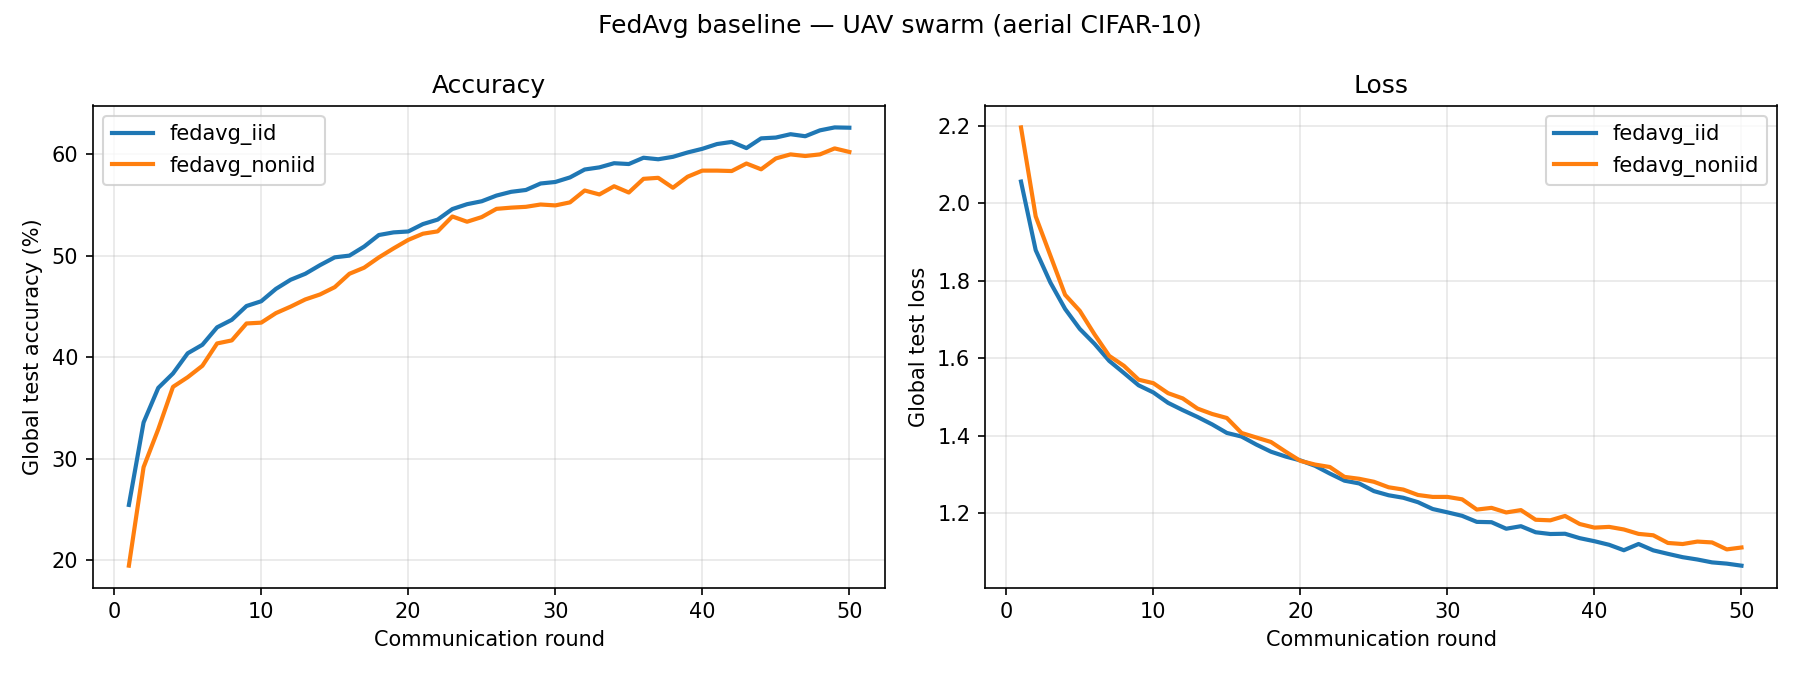
\includegraphics[width=\textwidth]{baseline_curves.png}
\caption{Test accuracy and loss of the FedAvg baseline over 50 rounds.}
\label{fig:baseline}
\end{figure}

Non-IID data cost about 2.4 percentage points, and neither curve had fully levelled
off by round 50. These accuracies are not direct targets for the later experiments,
which use 30 or 100 rounds, one local epoch and, in the controlled study, a
hierarchical system; robust methods are instead compared with matched clean controls
within each experiment.

\section{Preliminary Study Results}
The preliminary study compared FedAvg, the CosAvg-style baseline (inspired by
Liao et al.~\cite{liao2023tee}, not an exact reproduction) and an early version of CCRA with one
BS, 30 rounds, one local epoch and a single seed. Three of the ten UAVs flipped their
labels, and in the jammed scenarios a ground jammer targeted three honest UAVs.
Table~\ref{tab:prelim} lists the final accuracy (mean of the last five rounds), and
Figs.~\ref{fig:prelim-acc} and~\ref{fig:prelim-weight} show the accuracy and the
weight each method gave to the attackers.

\begin{table}[ht]
\centering
\caption{Preliminary study: final accuracy (\%), single seed, 30 rounds. CosAvg is our
CosAvg-style baseline, not the published method.}
\label{tab:prelim}
\begin{tabular}{@{}lccc@{}}
\toprule
Scenario & FedAvg & CosAvg & CCRA (early) \\
\midrule
No attack, ideal channel & 46.5 & \textbf{47.1} & 44.5 \\
No attack, jammed lossy channel & 44.6 & \textbf{45.6} & 43.1 \\
30\% label flip, ideal channel & 37.6 & 36.6 & \textbf{43.3} \\
30\% label flip, jammed lossy channel & 36.8 & 39.7 & \textbf{43.0} \\
\bottomrule
\end{tabular}
\end{table}

\begin{figure}[ht]
\centering
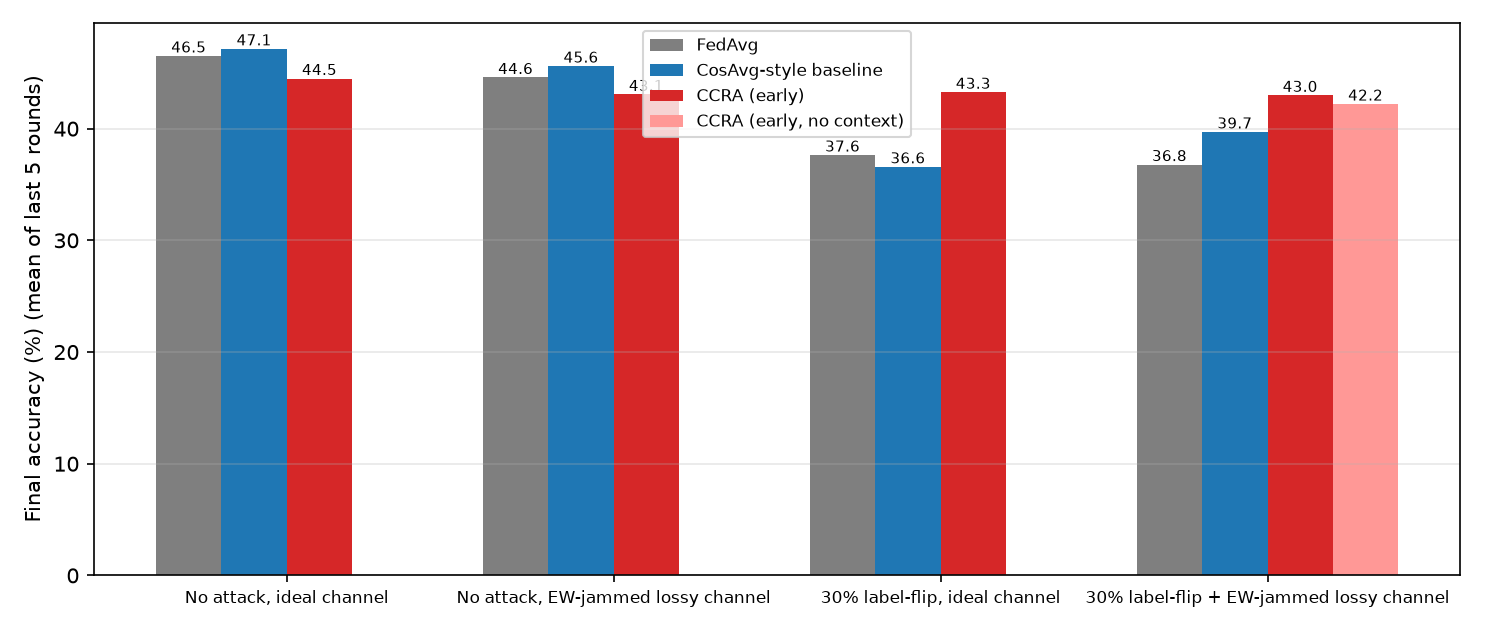
\includegraphics[width=\textwidth]{prelim_accuracy_bars.png}
\caption{Preliminary study: final accuracy in the four scenarios.}
\label{fig:prelim-acc}
\end{figure}

\begin{figure}[ht]
\centering
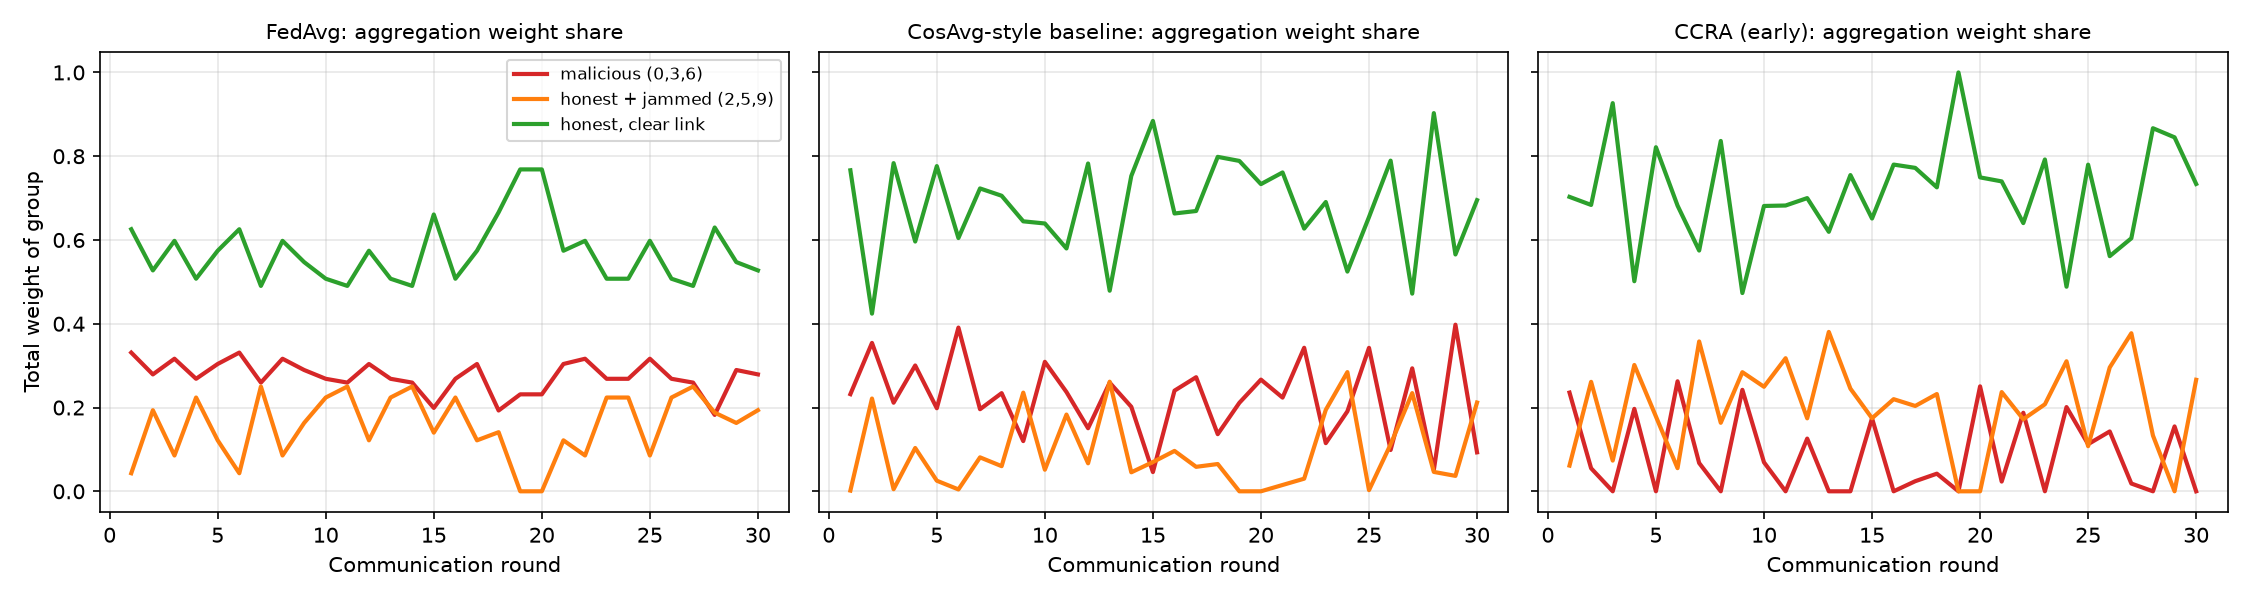
\includegraphics[width=0.9\textwidth]{prelim_weight_share.png}
\caption{Preliminary study: aggregation weight given to attackers and to jammed
honest UAVs under label flipping on the jammed channel.}
\label{fig:prelim-weight}
\end{figure}

The early CCRA kept about 43\% accuracy in both attacked scenarios. Averaged over
the last ten rounds, attackers received 1.9\% of its aggregation weight on the ideal
channel (CosAvg-style: 19.1\%; FedAvg: 26.0\%) and 8.4\% on the jammed lossy channel
(CosAvg-style: 21.5\%; FedAvg: 27.5\%). With no attack, early CCRA was 2.0 points
below FedAvg on the ideal channel and 1.5 points below it on the jammed channel;
the corresponding costs relative to the CosAvg-style baseline were 2.7 and 2.5 points.
These results were encouraging, but they could not support a claim:
\begin{itemize}
\item they came from one seed, so the size of the random variation was unknown;
\item the channel-aware part of CCRA added only 0.8 points over its no-context
  ablation (42.2 to 43.0\%), and with one seed the uncertainty in that difference
  could not be estimated;
\item CCRA used a trusted root set while CosAvg did not, so the comparison mixed two
  differences;
\item the reputation rule was revised when the system was extended to hierarchical
  FL, so the early CCRA is not the exact version evaluated in the controlled study.
\end{itemize}
The paired ablation isolates the effects of masking and telemetry.

\section{Controlled Ablation Study Results}
\label{sec:controlled}
Validation accounted for all \NumRuns{} planned outcomes, including numerical
divergences. The trace delivered on average \PdrTrace\% of packets at 15\,dB and
\PdrStress\% at 5\,dB. The two trace anchors share a geometry with neighbouring
base stations roughly 14\,m from the central station. The ideal condition instead
uses random walks and neighbours 240\,m from the centre. The change in conditions
also changes association behaviour: the ideal runs average \IdealHandovers{}
handovers, compared with \TraceHandovers{} per trace run. Comparisons with the
ideal setting therefore combine packet delivery, geometry and mobility effects.

\subsection{Stability and Overall Accuracy}
Table~\ref{tab:outcomes} pools all conditions to show divergence counts and overall
accuracy. Figure~\ref{fig:acc} restricts the accuracy comparison to attacked runs
and groups them by channel.

\begin{table}[ht]
\centering
\caption{Outcomes over all \NumRuns{} runs (120 per method). Diverged runs count as 10\%.}
\label{tab:outcomes}
\begin{tabular}{@{}lccc@{}}
\toprule
Method & Diverged & All runs (\%) & Attacked, 5\,dB (\%) \\
\midrule
FedAvg & 41/120 & 37.3 & 29.4 \\
Median & 26/120 & 29.3 & 21.3 \\
FLTrust & 0/120 & 50.6 & \textbf{50.1} \\
No-context & 0/120 & 51.4 & 45.3 \\
Mask-only & 0/120 & \textbf{52.8} & 49.5 \\
CCRA (full) & 0/120 & 51.1 & 46.0 \\
\bottomrule
\end{tabular}

\end{table}

\begin{figure}[ht]
\centering
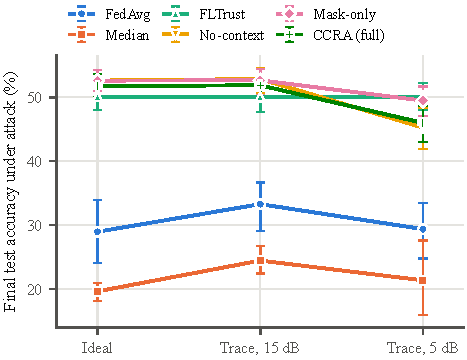
\includegraphics[width=0.75\textwidth]{accuracy_vs_channel.pdf}
\caption{Final accuracy under attack (mean over sign flip, ALIE and IPM and
\NumSeeds{} seeds). Error bars: 95\% seed-bootstrap intervals. Dashed, starred rules
are from the separate \BpNumRuns-run follow-up; cross-study rankings are descriptive.}
\label{fig:acc}
\end{figure}

FedAvg diverged in \DivFedavg{} and the coordinate-wise median in \DivMedian{} of
their 120 runs; FedAvg diverged in all 30 sign-flip runs. None of the four
methods that use a trusted reference update (FLTrust and the three CCRA variants)
diverged in its 120 runs. A plausible explanation for the median's failures, not
tested by a separate diagnostic, is that each cell holds only a few UAVs, so one
attacker in a cell is already a large fraction of the values being compared. Over all runs the mask-only variant has the highest accuracy,
\AllMask\%, against \AllFedavg\% for FedAvg. Table~\ref{tab:per-attack} breaks the
result down by attack.

\begin{table}[ht]
\centering
\caption{Final test accuracy averaged over seeds (\%). Within each attack setting,
bold marks the highest mean for each channel.}
\label{tab:per-attack}
\small
\begin{tabular}{@{}llccc@{}}
\toprule
Attack & Method & Ideal & Trace, 15 dB & Trace, 5 dB \\
\midrule
No attack & FedAvg & \textbf{59.2} & \textbf{59.3} & 54.1 \\
 & Median & 52.5 & 52.7 & 49.7 \\
 & FLTrust & 52.5 & 51.5 & 52.9 \\
 & No-context & 57.1 & 56.7 & 51.1 \\
 & Mask-only & 57.1 & 57.5 & \textbf{54.7} \\
 & CCRA (full) & 55.4 & 56.6 & 52.6 \\
\midrule
Sign flip & FedAvg & 10.0 & 10.0 & 10.0 \\
 & Median & 10.0 & 19.6 & 12.4 \\
 & FLTrust & 50.0 & 49.9 & \textbf{50.6} \\
 & No-context & \textbf{54.2} & \textbf{53.8} & 46.1 \\
 & Mask-only & 54.2 & 53.6 & 49.9 \\
 & CCRA (full) & 52.5 & 52.8 & 46.5 \\
\midrule
ALIE & FedAvg & 49.8 & 46.9 & 42.0 \\
 & Median & 35.4 & 28.4 & 28.1 \\
 & FLTrust & 49.9 & 50.6 & 49.6 \\
 & No-context & \textbf{52.9} & 52.6 & 46.0 \\
 & Mask-only & 52.9 & \textbf{52.7} & \textbf{50.8} \\
 & CCRA (full) & 52.8 & 51.9 & 46.9 \\
\midrule
IPM & FedAvg & 27.0 & 42.9 & 36.0 \\
 & Median & 13.4 & 25.3 & 23.5 \\
 & FLTrust & 50.5 & 49.7 & \textbf{50.0} \\
 & No-context & \textbf{50.7} & \textbf{52.3} & 43.6 \\
 & Mask-only & 50.7 & 51.7 & 47.7 \\
 & CCRA (full) & 50.0 & 51.0 & 44.5 \\
\bottomrule
\end{tabular}

\end{table}

Two points in Table~\ref{tab:per-attack} deserve attention. First, with no attack,
plain FedAvg is the most accurate method on the ideal and 15\,dB channels; every
robust method pays a cost of roughly two to eight points for discarding or
down-weighting honest updates. Second, on the 5\,dB channel the masked variant is
slightly ahead of FedAvg even without an attack, consistent with FedAvg's zero-filled
lost coordinates now hurting it.

\subsection{Which Kind of Channel Awareness Helps}
Figure~\ref{fig:ablation} shows the paired contrasts that separate the two channel
mechanisms.

\begin{figure}[ht]
\centering
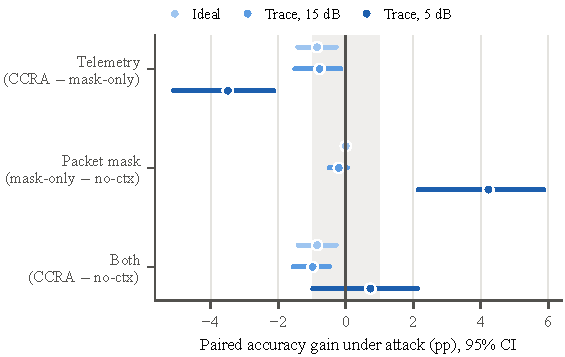
\includegraphics[width=0.75\textwidth]{ablation_contrasts.pdf}
\caption{Paired accuracy differences under attack with 95\% bootstrap intervals. The
grey band is the prespecified $\pm1$ point region of practical equivalence.}
\label{fig:ablation}
\end{figure}

\textbf{Erasure masking.} On the ideal channel nothing is lost, so mask-only and
no-context are identical. As the link weakens the masks matter more, and at 5\,dB
masking adds \MaskGain{} points over the no-context baseline, which treats lost
packets as zeros (95\% CI \ci{\MaskLo}{\MaskHi}). Treating lost
coordinates as zeros shrinks honest updates, distorts their similarity scores and
pulls the average towards zero; ignoring them avoids all three effects.

\textbf{Telemetry in the reputation.} The prespecified primary estimate, the
telemetry effect at 5\,dB minus that at 15\,dB, is $\PrimGain$ points
(\ci{\PrimLo}{\PrimHi}). Even the upper bound falls below $-1$ point, meeting the
prespecified criterion for an additional accuracy penalty at the weaker anchor.
At 5\,dB, full CCRA scored \AccCcraStress\% and mask-only scored
\AccMaskStress\%, a gap of $\TelGain$ points (\ci{\TelLo}{\TelHi}). In the
attacked ideal runs, where delivery is complete, the gap is $\TelIdeal$ points.

\textbf{Both together.} Full CCRA against no-context combines a gain and a loss; at
5\,dB the net effect is small and its interval includes the equivalence region. The
earlier impression that ``channel context helps'' came from this combination, which
hid two opposite effects.

\subsection{Mechanism: Who the Gate Rejects}
\label{sec:mechanism}
Section~\ref{sec:fixed-point} predicted that slowing rewards on weak links would push
honest UAVs' reputations down without doing much to attackers.
Figure~\ref{fig:gate} is consistent with that pattern.

\begin{figure}[ht]
\centering
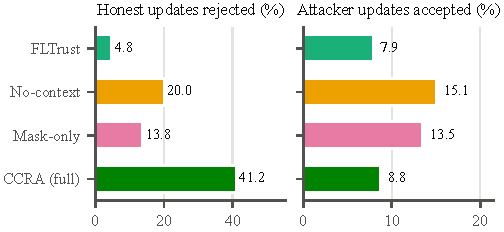
\includegraphics[width=0.75\textwidth]{gate_rates.pdf}
\caption{Gate decisions under attack at 5\,dB, as a percentage of received updates,
averaged over attacks and seeds.}
\label{fig:gate}
\end{figure}

With telemetry, the gate rejected \RejCcra\% of honest updates against \RejMask\%
without it, while the share of attacker updates accepted fell only from \AccptMask\%
to \AccptCcra\%. The accuracy loss from telemetry was accompanied by this rise in
honest-update rejection. The rule gave up a large amount of honest data to filter slightly
more attacker data, and it did so precisely when honest data were already scarce
because of packet loss. These rates are descriptive. They agree with the analysis in
Section~\ref{sec:fixed-point}, but they do not by themselves prove that it is the
cause.

\subsection{Comparison with FLTrust}
At the 5\,dB anchor under attack, FLTrust exceeds full CCRA by
\FltOverCcraStress{} points (\AccFltrustStress\% versus \AccCcraStress\%;
Table~\ref{tab:outcomes}). FLTrust is the closest established method, since it uses
the same root set, although with more root training steps. Its gate
rejected only \RejFltrust\% of honest updates at 5\,dB. It has no reputation memory,
since each round is judged on its own, but its norm matching, score normalization,
weights and gating also differ from CCRA's, so the lower rejection cannot be
attributed to memory alone. In an exploratory paired comparison, mask-only was
\VsFltTrace{} points better than FLTrust under attack at 15\,dB
(\ci{\VsFltTraceLo}{\VsFltTraceHi}), while the 5\,dB comparison was inconclusive
($\VsFltStress$ points, \ci{\VsFltStressLo}{\VsFltStressHi}): the interval supports
neither a difference nor practical equivalence, since it is not entirely inside
$\pm1$ point. The different root training budgets and aggregation rules also
limit what this comparison can establish about reputation memory.

\section{Completed Base-Paper Comparison}
\label{sec:bp-results}
The \BpNumRuns{} terminal outcomes comprise 157 successful runs and 83 numerical
divergences. Fresh-only diverged in \BpDivFresh{} of 120 runs, and reuse-old in
\BpDivReuse{} of 120. All 60 sign-flip runs diverged; the remaining 23 divergences
occurred under IPM. No clean or ALIE run diverged. These outcomes are retained at
10\% final accuracy, rather than excluded or retried into successful runs.
All-run accuracy is \BpAllFresh\% for fresh-only and \BpAllReuse\% for reuse-old.

\begin{table}[ht]
\centering
\caption{Separate base-paper follow-up: ten paired seeds per cell. Final accuracy
includes numerical divergences at chance (10\%). Intervals are exploratory paired
seed-bootstrap intervals, with no multiplicity adjustment.}
\label{tab:bp-results}
\small
\begin{tabular}{@{}llrrr@{}}
\toprule
Attack & Channel & Fresh (\%) & Reuse (\%) & Fresh $-$ reuse: pp [95\% CI] \\
\midrule
No attack & Ideal & 59.0 & 59.0 & $+0.0\;[+0.0,\,+0.0]$ \\
 & 15\,dB & 59.4 & 59.4 & $+0.0\;[-0.2,\,+0.3]$ \\
 & 5\,dB & 56.9 & 51.5 & $+5.4\;[+4.1,\,+6.7]$ \\
\midrule
Sign flip & Ideal & 10.0 & 10.0 & $+0.0\;[+0.0,\,+0.0]$ \\
 & 15\,dB & 10.0 & 10.0 & $+0.0\;[+0.0,\,+0.0]$ \\
 & 5\,dB & 10.0 & 10.0 & $+0.0\;[+0.0,\,+0.0]$ \\
\midrule
ALIE & Ideal & 49.7 & 49.5 & $+0.2\;[+0.0,\,+0.3]$ \\
 & 15\,dB & 47.2 & 47.2 & $+0.0\;[-0.3,\,+0.3]$ \\
 & 5\,dB & 43.3 & 39.8 & $+3.5\;[+0.5,\,+6.5]$ \\
\midrule
IPM & Ideal & 26.9 & 26.9 & $+0.0\;[-0.1,\,+0.0]$ \\
 & 15\,dB & 42.9 & 42.9 & $+0.0\;[-0.1,\,+0.2]$ \\
 & 5\,dB & 37.5 & 30.8 & $+6.7\;[+1.4,\,+15.0]$ \\
\bottomrule
\end{tabular}

\end{table}

Table~\ref{tab:bp-results} shows identical mean accuracy on the clean ideal channel,
where there are no missing packets to reuse. On clean stressed links, fresh-only
attains \BpCleanStressFresh\% versus \BpCleanStressReuse\% for reuse-old: a gain of
\BpCleanGain{} percentage points (95\% CI \ci{\BpCleanLo}{\BpCleanHi}). Under attack
at 5\,dB, the chance-scored means are \BpAttackStressFresh\% and
\BpAttackStressReuse\%, respectively, a gain of \BpAttackGain{} points
(\ci{\BpAttackLo}{\BpAttackHi}). The interval describes a mean over the three
attacks within each seed, not 30 independent replicates.

Retaining old parameters does not improve this finite-horizon stressed-channel
experiment, and neither rule provides Byzantine robustness. This is compatible with
the scope of Shirvanimoghaddam et al.~\cite{shirvanimoghaddam2022erroneous}: its analysis assumes honest
clients and whole-upload erasures, whereas the present implementation uses packet
erasures in a hierarchical non-IID CNN task with adversarial updates. These results
are an adaptation study, not an exact reproduction or a refutation of the original
convergence theorem.

Figure~\ref{fig:acc} now includes both rules alongside the original six methods.
The original ablation's findings about masking and telemetry are unchanged.

\subsection{Our Method against the Base Paper}
\label{sec:vs-bp}
Both studies use the same seeds, data partitions and attacker identities, so mask-only
CCRA can be compared with the base paper's better rule, fresh-only, seed by seed. Under
attack at 5\,dB, mask-only attains \AccMaskStress\% against \BpAttackStressFresh\% for
fresh-only, a paired gain of \VsBpAttack{} percentage points (95\% CI
\ci{\VsBpAttackLo}{\VsBpAttackHi}). Without attack at 5\,dB, fresh-only is ahead,
\BpCleanStressFresh\% against \AccMaskCleanStress\%, a signed difference of $\VsBpClean$ points
(\ci{\VsBpCleanLo}{\VsBpCleanHi}); the signed contrast is mask-only minus fresh-only.
FLTrust, which also uses a trusted reference, scored \FltVsBpAttack{} points
above fresh-only in the attacked 5\,dB comparison. Fresh-only already restricts
its average to delivered coordinates. Both contrasts also include differences
in scoring and weighting. The controlled comparison with zero-filled no-context
CCRA estimates the effect of masking separately.

The two studies ran on different hardware (an A100 against RTX~2060 and GTX~1650
workers) and software versions, so these contrasts are cross-study and exploratory.
Complete delivery makes fresh-only equivalent to FedAvg, giving us a cross-check
on the ideal runs. The same runs diverged in both studies. For the \XcheckRuns{}
remaining ideal pairs, the absolute accuracy difference averaged \XcheckMean{}
points and reached at most \XcheckMax{} points. This check measures agreement only
under complete delivery. The hardware contribution to the 5\,dB comparison
remains unmeasured.

The coordinator recovered interrupted jobs separately from the divergence analysis.
It verified the checkpoints before requeuing clean stops recorded as application
failures. Windows progress-file permission errors triggered bounded retries with
the same experiment settings. The audit history retains the failed attempts, and
validation accepted exactly one terminal record for each planned job. A resumed job
restores the saved training and random-generator states. Bitwise agreement between
GPUs was outside the scope of that validation.

\section{Discussion}
\subsection{What the Results Show}
\begin{enumerate}
\item FLTrust and the three CCRA variants completed all 480 runs without
  numerical divergence. The root set is one of several design choices that
  distinguish these methods from FedAvg and the median.
\item In the attacked trace runs, masking adds little at 15\,dB, where nearly
  every packet arrives. At 5\,dB, it raises accuracy by \MaskGain{} points.
  The study measured accuracy and stability. The computational and communication
  costs of masking remain unmeasured.
\item At 5\,dB, telemetry slowed trust recovery while the penalty for a low score
  stayed the same. The drift calculation in Section~\ref{sec:fixed-point} predicts
  that this asymmetry lowers equilibrium trust as evidence weakens.
\item In the erasure-rule follow-up, fresh-only gave higher accuracy at 5\,dB
  than reuse-old. Every sign-flip run diverged with either rule, even with
  packet-level erasure handling.
\end{enumerate}

\subsection{Why a Negative Result Is Useful}
The preliminary study suggested that CCRA's channel context was its key ingredient.
Had that claim been carried forward, Phase~II would have been built on a component
that harms accuracy. The prespecified design, paired seeds and chance scoring of
diverged runs made it possible to reject the claim with confidence, and the
analysis in Section~\ref{sec:fixed-point} points to the specific rule that must
change.

\subsection{Threats to Validity}
\begin{itemize}
\item \textbf{Channel realism.} The trace comes from one measured BS; the other BSs
  are virtual, and the 5 and 15\,dB anchors are assumptions, not calibrated values.
  The virtual neighbours are about 14\,m from the reference BS (about 28\,m from
  each other). In the separate 60-round channel validation, the median SNR at
  the nominal 5\,dB anchor is 8.6\,dB, not 5\,dB. There are no retransmissions.
  The trace replays average \TraceHandovers{} handovers. Comparisons with the
  ideal condition also reflect the different geometry and association patterns.
  The effect of frequent handovers in trace replay remains an open question.
\item \textbf{Scope of learning task.} The experiment uses one CNN trained on
  transformed CIFAR-10 images as a proxy for aerial imagery. The swarm size and
  attack strengths are fixed.
\item \textbf{Trust assumptions.} The simulation gives each BS access to a root
  set assumed to be clean. It leaves trusted execution and attestation to a future
  implementation.
\item \textbf{Attacker model.} The comparison assumes authentic telemetry and
  fixed poisoning strategies. An adaptive attacker that targets trust over
  multiple rounds, as studied by Liu et al.~\cite{liu2026evade}, is outside this
  design.
\item \textbf{Statistics.} Intervals reflect ten paired seeds. Secondary contrasts
  use unadjusted intervals. Phase~II confirmation requires fresh seeds.
\item \textbf{Execution environment.} The A100 ablation and Windows-worker follow-up
  used different GPU/software profiles and source fingerprints. Checkpoint recovery
  was verified, but hardware-controlled cross-study effects and runtime speedups
  were not measured.
\end{itemize}
